\section{内部排序}

\begin{frame}[plain]
  \begin{outlinebox}{内部排序大纲}
    \begin{itemize}
    \item 排序的基本概念
    \item 具体排序方法
      \begin{enumerate}
      \item \color{red} 插入排序:直接插入排序
      \item 插入排序:折半插入排序
      \item 插入排序:希尔排序
        
      \item \color{blue} 交换排序:冒泡排序
      \item 交换排序:快速排序
        
      \item \color{orange} 选择排序:简单选择排序
      \item 选择排序:堆排序
        
      \item \color{purple} 归并排序:二路归并
      \item \color{gray} 基数排序
      \end{enumerate}
    \end{itemize}    
  \end{outlinebox}
\end{frame}

\subsection{排序的基本概念}
\begin{frame}[fragile]
  \frametitle{排序}
  \begin{easylist} \easyitem

    & 对一个数据元素集合或序列重新排列成一个按数据元素某个项值有序的序列就是排
    序。

    && 例如将关键字序列:

    $52, 49, 80, 36, 14, 58, 61, 23, 97, 75$

    调整为
    
    $14, 23, 36, 49, 52, 58, 61 ,75, 80, 97$

    && 再如将:

    $<Susie,26>, <Jack,22>, <Michel,25>, <Richard,25>$

    调整为:

    $<Jack,22>,<Michel,25>, <Richard, 25>, <Susie,26>$
  \end{easylist}
\end{frame}

\begin{frame}[fragile]
  \frametitle{排序的稳定性}
  \begin{easylist} \easyitem

    & 请注意刚才第二个序列的排序结果不唯一!

    $<Susie,26>, <Jack,22>, <Michel,25>, <Richard,25>$

    \color{red} $<Jack,22>,<Michel,25>, <Richard, 25>, <Susie,26>$

    \color{blue} $<Jack,22>, <Richard, 25>, <Michel,25>, <Susie,26>$
    
    & \color{red}排序算法的稳定性

    && 若存在相同的关键字,对应位置的记录在排序后仍然保持原来的顺序,则称所使用的排
    序方法是稳定的。反之称为不稳定的。

  \end{easylist}
\end{frame}

\subsection{插入排序}
\begin{frame}[fragile]
  \frametitle{}
  \begin{sectionbox}{插入排序}
    \begin{itemize}
    \item 直接插入排序
    \item 折半插入排序
    \item 希尔排序
    \end{itemize}
  \end{sectionbox}
\end{frame}

\subsubsection{直接插入排序}
\begin{frame}[fragile]
  \frametitle{直接插入排序}

  对于要插入的元素$R[i]$,从$R[i-1]$起向前进行顺序查找,当$R[j-1]$小于$R[i]$时停止,插
  入位置为$R[j]$。注意在顺序表中要移动元素实现元素的插入。

  \begin{center}
    \begin{tikzpicture}[box/.style={draw, fill=green!20, minimum size=1cm}]
      \draw[draw] node[box, fill=red!20] (b0) {76}
      node[box, right=0 of b0] (b1) {38} 
      node[box, right=0 of b1] (b2) {49}
      node[box, right=0 of b2] (b3) {65}
      node[box, right=0 of b3] (b4) {97}
      node[box, right=0 of b4, fill=blue!10] (b5) {76}
      node[box, right=0 of b5, fill=blue!10] (b6) {13}
      node[box, right=0 of b6, minimum width=2cm, fill=blue!10] (b7) {$\cdots$}; 

      \foreach \i in {0,...,6}
      {
        \draw node[above=0 of b\i] (idx_\i) {$\i$};
      };

      \draw node[above=0 of idx_5] {$R[i]$} node[above=0 of idx_0] {$R[0]$};

      \path[] (b0.south) ++(0,-1.5cm) edge[-Latex, dashed] node[below, align=center]{设置“哨兵”存储$R[i]$,\\只要待比较的元素大于$R[0]$,\\就继续往前比较,从而实现\\$R[j] \cdots R[i-1]$的后移。} (b0.south);

      \path[] (b4.south) ++(0,-1.5cm) edge[-Latex, very thick, draw=red] node[below right,align=center]{$j$, 指示插入的位置,\\$R[j-1] \leq R[i]$  \\ (稳定的排序方法)} (b4.south);
    \end{tikzpicture}
  \end{center} 
\end{frame}

\begin{frame}[fragile]
  \frametitle{直接插入排序举例}

  \begin{center}
    \begin{tabular}{ c c c c c c c }
      \toprule
      47 & 38 & 65 & 97 & 13 & 27 & \circled{47} \pause \\ \midrule 
      \cellcolor{blue!20} 47 & \cellcolor{red!20} 38 & 65 & 97 & 13 & 27 & \circled{47} \pause \\ \midrule
      \cellcolor{blue!20} 38 &  \cellcolor{blue!20} 47 & \cellcolor{red!20} 65 & 97 & 13 & 27 & \circled{47} \pause \\ \midrule
      \cellcolor{blue!20} 38 &  \cellcolor{blue!20} 47 &  \cellcolor{blue!20} 65 & \cellcolor{red!20} 97 & 13 & 27 & \circled{47} \pause \\ \midrule
      \cellcolor{blue!20} 38 &  \cellcolor{blue!20} 47 &  \cellcolor{blue!20} 65 & \cellcolor{blue!20} 97 & \cellcolor{red!20} 13 & 27 & \circled{47} \pause \\ \midrule
      \cellcolor{blue!20} 13 &  \cellcolor{blue!20} 38 &  \cellcolor{blue!20} 47 & \cellcolor{blue!20} 65 & \cellcolor{blue!20} 97 & \cellcolor{red!20} 27 & \circled{47} \pause \\ \midrule
      \cellcolor{blue!20} 13 &  \cellcolor{blue!20} 27 &  \cellcolor{blue!20} 38 & \cellcolor{blue!20} 47 & \cellcolor{blue!20} 65 & \cellcolor{blue!20} 97 & \cellcolor{red!20} \circled{47} \pause \\ \midrule
      \cellcolor{blue!20} 13 &  \cellcolor{blue!20} 27 &  \cellcolor{blue!20} 38 & \cellcolor{blue!20} 47 & \cellcolor{blue!20} \circled{47} & \cellcolor{blue!20} 65 & \cellcolor{blue!20} 97 \\ \bottomrule
    \end{tabular}
  \end{center}

  注意:两个47的位置(带有圆圈和不带有圆圈)。
\end{frame}

\begin{frame}[fragile]
  \frametitle{直接插入排序算法分析}
  \begin{easylist} \easyitem
    & 空间效率: 用一个辅助单元

    & 时间效率: 时间复杂度为$O(n^2)$
    
    && 进行了n-1次向有序表插入记录的操作,每趟是“比较+移动”

    && 最好情况:记录按关键字正序

    &&& $n-1$次比较,$0$次移动

    && 最差情况:记录按关键字逆序
    
    &&& 比较次数:
    $\sum_{i=2}^n i = 2+3+\cdots + n = \dfrac{(n+2) \times (n-1)}{2}$
    
    &&& 移动次数:
    $\sum_{i=2}^n (i+1) = \dfrac{(n+4) \times (n-1)}{2}$

    && 平均情况:不妨取上述各值的平均,可知比较和移动次数约$n^2/4$

    & 是稳定的排序方法
  \end{easylist}
\end{frame}


\subsubsection{希尔排序}
\begin{frame}[fragile]
  \frametitle{希尔(Shell)排序}
  \begin{infobox}{希尔排序的思想}
    对于元素数量较少,或者基本有序的待排序序列,直接插入排序的效率不错。
   \end{infobox}

  \begin{easylist} \easyitem
    & 根据增量$d$分割出子序列
    
    & 对子序列进行直接插入排序

    & 增量$d$的选择

    && Shell最初的方案:
    $d = n/2, d=d/2, \cdots , d=1$

    && Knuth的方案:
    $d=d/3 + 1$

    && 其它:d为奇数; d互质 $\cdots$
  \end{easylist}
\end{frame}

\begin{frame}[fragile, allowframebreaks]
  \frametitle{希尔排序举例}
  \begin{infobox}{第1趟:$d_1=5$}
    \begin{center}
      \begin{tabular}{|c|c|c|c|c|c|c|c|c|c|}
        \hline
        \rowcolor{yellow!50}
        \circled[red]{49} & 38 & 65  & 97 & 76 & 13 & 27 & \circled{49} & 55 & 04 \\ \hline
        13 & ~   &    &    &    & \circled[red]{49} &    &    &    &     \\ \hline
        ~ & 27   &    &    &    &    & 38 &    &    &     \\ \hline
        ~ &      & \circled{49} &    &    &    &    & 65 &    &     \\ \hline
        ~ &      &    & 55 &    &    &    &    & 97 &     \\ \hline
        ~ &      &    &    & \cellcolor{red!5} 04 &    &    &    &    & 76  \\ \hline
      \end{tabular}
    \end{center}
  \end{infobox}

  \begin{easylist} \easyitem
    & 观察04: 跳跃式的往前移
    & 观察49: 希尔排序不稳定
  \end{easylist}

  \newpage

  \begin{infobox}{第2趟:$d_2=2$}
    \begin{center}
      \begin{tabular}{|c|c|c|c|c|c|c|c|c|c|}
        \hline
        \rowcolor{yellow!50}
        13 & 27  &  \circled{49}  & 55   & 04 & \circled[red]{49}  &  38  &  65  &  97  & 76  \\ \hline
        04 &     &  13  &    &  38 &      & \circled{49} &    &  97  &      \\ \hline
        ~ &  27   &    & \circled[red]{49}   &    &  55  &  &  65  &    & 76    \\ \hline
      \end{tabular}
    \end{center}
  \end{infobox}

  \pause
  
  \begin{infobox}{第3趟:$d_3=1$}
    \begin{center}
      \begin{tabular}{|c|c|c|c|c|c|c|c|c|c|}
        \hline
        \rowcolor{yellow!50}
        04 & 27  & 13 &  \circled[red]{49}  & 38 & 55 & \circled{49}  &  65  &  97  & 76  \\ \hline
        04 & 13  & 27 &  38 & \circled[red]{49}  & \circled{49} & 55 &  65  &  76  & 97  \\ \hline
      \end{tabular}
    \end{center}
  \end{infobox}
\end{frame}

\begin{frame}[fragile]
  \frametitle{希尔排序分析}
  \begin{easylist} \easyitem
    & 希尔排序的时间性能优于直接插入排序!
    
    & 希尔排序开始时增量$d$较大(这使得分组较多,每组记录少),故各组内直接插入较
    快,后来增量$d$渐小(各组记录渐多),但组内元素已经比较接近有序状态,所以新的一趟
    排序过程也比较快。

    & 希尔排序的复杂度分析很复杂

    && 在特定情况下可以准确估算比较、移动次数,但是考虑与增量之间的依赖关系,并给出
    完整的数学分析,目前还做不到

    && 在增量序列为$\delta[k]=2^{t-k+1}$时, 希尔排序的时间复杂度为$O(n^{3/2})$
    
    && Knuth的统计结论是,平均比较次数和对象平均移动次数在$n^{1.25}$与$1.6 \cdot
    n^{1.25}$之间。    
  \end{easylist}
\end{frame}

\begin{frame}[plain]
  \vspace{2cm}
  \begin{infobox}{希尔排序增量序列的取法}
    目前尚未有工作求得一种最好的增量序列。但需注意的是:应使增量序列中的值没有
    除1之外的公因子,并且最后一个增量必须为1。
  \end{infobox}
\end{frame}

\begin{frame}[fragile]
  \frametitle{练习}
  分析以下关键字的希尔排序过程:

  \begin{center}
    \begin{tikzpicture}[box/.style={draw, minimum size=0.6cm, minimum width=1cm}]
      \draw node (b0) {};
      \foreach[count=\i, evaluate=\i as \idx using int(\i-1)] \e in {47,38,47,9,78,13,27,66}
      {
        \draw node[right=0 of b\idx, box] (b\i) {$\e$};
        \draw node[above=0 of b\i] {$\idx$};
      };
    \end{tikzpicture}
  \end{center}
\end{frame}


\subsection{交换排序}
\begin{frame}[fragile]
  \frametitle{}
  \begin{sectionbox}{交换排序}
    \begin{itemize}
    \item 冒泡排序
    \item 快速排序
    \end{itemize}
  \end{sectionbox}
\end{frame}

\subsubsection{冒泡排序}
\begin{frame}[fragile, allowframebreaks]
  \frametitle{冒泡排序(Bubble Sort)}
  \begin{infobox}{算法思想}
    比较相邻两个结点,较大的结点往下移,较小的往上移,使得每轮比较结束后最大的沉到最
    后.
  \end{infobox}

  \newpage
  
  \begin{center}
    \begin{tabular}{|p{0.6cm}|p{0.6cm}|p{0.6cm}|p{0.6cm}|p{0.6cm}|p{0.6cm}|p{0.6cm}|}
      \hline
      49 & 38 & 38 & 38 & 38 & 13 & \cellcolor{red!15} 13 \\
      38 & 49 & 49 & 49 & 13 & 27 & \cellcolor{red!15} 27 \\
      65 & 65 & 65 & 13 & 27 & 38 & \cellcolor{red!15} 38 \\
      97 & 76 & 13 & 27 & 49 & \cellcolor{red!15} 49 & ~ \\
      76 & 13 & 27 & 49 & \cellcolor{red!15} 49 & ~  & ~ \\
      13 & 27 & 49 & \cellcolor{red!15}  65 &    &    &   \\
      27 & 49 & \cellcolor{red!15}  76 &    &    &    &   \\
      49 & \cellcolor{red!15} 97 &    &    &    &    &   \\
      \hline  
    \end{tabular}
  \end{center}
  第1列为原始序列;第2列为第1趟排序后的结果,第3列为第2趟排序后结果 $\cdots$

  最后一个数字为本趟排序挑选出的最大数字。
\end{frame}

\begin{frame}[fragile]
  \frametitle{冒泡排序算法分析}
  \begin{easylist} \easyitem
    & 最好情况下,初始状态是递增有序的

    && 扫描一趟,关键字的比较次数为$n-1$,记录移动0次

    & 最坏情况下,初始状态是反序的

    && 扫描$n-1$趟,第i趟扫描要进行$n-i$次关键字的比较,每次比较后进行记录移动,故有:

    比较次数: $\sum_{i=1}^{n-1}(n-i)=\dfrac{n \times (n-1)}{2}$

    移动次数: $\sum_{i=1}^{n-1}3(n-i)=\dfrac{3 \times n \times (n-1)}{2}$
    
    & 稳定的
  \end{easylist}
\end{frame}

\subsubsection{快速排序}

\begin{frame}[fragile]
  \frametitle{快速排序—冒泡法的改进}
  \begin{infobox}{算法思想}
    通过一趟排序将待排序记录分割成独立的两部分,其中一部分的关键字均小于另一部分的
    关键字,然后分别对这两部分记录继续分别进行排序即可。
  \end{infobox}

  \begin{center}
    \begin{tikzpicture}[box/.style={draw, minimum size=1cm},
      block/.style={draw=red, thick, dashed, minimum height=1.3cm}
      ]
      \draw[draw] node[box] (b0) {27}
      node[box, right=0 of b0] (b1) {38} 
      node[box, right=0 of b1] (b2) {13}
      node[box, right=0 of b2, fill=green!20] (b3) {49}
      node[box, right=0 of b3] (b4) {76}
      node[box, right=0 of b4] (b5) {97}
      node[box, right=0 of b5] (b6) {65}
      node[box, right=0 of b6] (b7) {49}
      node[block, right=-0.2cm of b0.west, minimum width=3.4cm] (bl) {}
      node[block, right=-0.2cm of b4.west,minimum width=4.4cm] (bl) {}
      ; 

      \foreach \i in {0,...,7}
      {
        \draw node[above=0 of b\i] (idx_\i) {$\i$};
      };
    \end{tikzpicture}
  \end{center}

  SEE: \url{https://www.itcodemonkey.com/article/11276.html}
\end{frame}

\begin{frame}[plain]
  \begin{infobox}{快速排序举例(单次划分过程)}
    \scalebox{0.8}{
      \begin{tikzpicture}[box/.style={draw, minimum size=0.6cm, minimum width=1cm},
        done/.style={fill=blue!5}]

        \draw node[] (b0) {};
        \foreach[count=\i, evaluate=\i as \leftx using int(\i-1)] \y in {49,38,65,97,76,13,27,49}
        {
          \draw node[box, right=0 of b\leftx] (b\i) {$\y$};
          \draw node[above=0 of b\i] (idx_\i) {$\leftx$};
        };
        \draw node[box, right=0 of b0, fill=red!20] (b1) {49};

        \draw[-Latex, draw=blue, thick] (b1.south) ++ (0,-0.7cm) -> (b1.south);
        \path (b8.south) ++ (0,-0.5cm) edge[-Latex, draw=red] node[right]{\textcircled{1}} (b8.south);
        \path (b7.south) ++ (0,-0.5cm) edge[-Latex, draw=red] node[right]{\textcircled{2}} (b7.south);

        \pause
        
        \draw node[below=1.2cm of b0] (b0) {}
        node[box, right=0 of b0, done] (b1) {27}
        node[box, right=0 of b1] (b2) {38}
        node[box, right=0 of b2] (b3) {65}
        node[box, right=0 of b3] (b4) {97}
        node[box, right=0 of b4] (b5) {76}
        node[box, right=0 of b5] (b6) {13}
        node[box, right=0 of b6, fill=red!20] (b7) {49}
        node[box, right=0 of b7, done] (b8) {49};


        \draw[-Latex, draw=blue, thick] (b1.south) ++ (0,-0.7cm) -> (b1.south);
        \path (b2.south) ++ (0,-0.5cm) edge[-Latex, draw=red] node[right]{\textcircled{1}} (b2.south);
        \path (b3.south) ++ (0,-0.5cm) edge[-Latex, draw=red] node[right]{\textcircled{2}} (b3.south);

        \pause

        \draw node[below=1.2cm of b0] (b0) {}
        node[box, right=0 of b0, done] (b1) {27}
        node[box, right=0 of b1, done] (b2) {38}
        node[box, right=0 of b2, fill=red!20] (b3) {49}
        node[box, right=0 of b3] (b4) {97}
        node[box, right=0 of b4] (b5) {76}
        node[box, right=0 of b5] (b6) {13}
        node[box, right=0 of b6, done] (b7) {65}
        node[box, right=0 of b7, done] (b8) {49};

        \draw[-Latex, draw=blue, thick] (b3.south) ++ (0,-0.7cm) -> (b3.south);
        \path (b6.south) ++ (0,-0.5cm) edge[-Latex, draw=red] node[right]{\textcircled{1}} (b6.south);

        \pause

        \draw node[below=1.2cm of b0] (b0) {}
        node[box, right=0 of b0, done] (b1) {27}
        node[box, right=0 of b1, done] (b2) {38}
        node[box, right=0 of b2, done] (b3) {13}
        node[box, right=0 of b3] (b4) {97}
        node[box, right=0 of b4] (b5) {76}
        node[box, right=0 of b5,fill=red!20] (b6) {49}
        node[box, right=0 of b6, done] (b7) {65}
        node[box, right=0 of b7, done] (b8) {49};

        \draw[-Latex, draw=blue, thick] (b6.south) ++ (0,-0.7cm) -> (b6.south);
        \path (b4.south) ++ (0,-0.5cm) edge[-Latex, draw=red] node[right]{\textcircled{1}} (b4.south);

        \pause

        \draw node[below=1.2cm of b0] (b0) {}
        node[box, right=0 of b0, done] (b1) {27}
        node[box, right=0 of b1, done] (b2) {38}
        node[box, right=0 of b2, done] (b3) {13}
        node[box, right=0 of b3,fill=red!20] (b4) {49}
        node[box, right=0 of b4] (b5) {76}
        node[box, right=0 of b5, done] (b6) {97}
        node[box, right=0 of b6, done] (b7) {65}
        node[box, right=0 of b7, done] (b8) {49};

        \draw[-Latex, draw=blue, thick] (b4.south) ++ (0,-0.7cm) -> (b4.south);
        \path (b5.south) ++ (0,-0.5cm) edge[-Latex, draw=red] node[right]{\textcircled{1}} (b5.south);
        \path (b4.south) ++ (0.2cm,-0.5cm) edge[-Latex, draw=red] node[right]{\textcircled{2}} (b4.-60);
      \end{tikzpicture}
    }

    其中:带圆圈的数字表示比较的次序;蓝色箭头表示枢轴元素的位置;红色箭头表示要
    比较的元素位置。
  \end{infobox}
\end{frame}

\begin{frame}[fragile]
  \frametitle{快速排序算法分析}
  \begin{easylist} \easyitem
    & 空间效率

    && 快速排序是递归的,递归调用层次数与上述二叉树的深度一致。因而存储开销在理想
    情况下为$O(log_2 n)$,即树的高度;最坏情况下为$O(n)$,即二叉树是一个单链

    & 时间效率

    && 对于$n$个记录的待排序列,一次划分需要$n-1$次比较,时效为$O(n)$,若设$T(n)$为对$n$个记录
    的待排序列进行快速排序所需时间

    && 理想情况下:每次划分正好将分成两个等长的子序列

    \[T(n) \leq cn+2T(n/2) \cdots = O(n log_2n)\]
    & 最坏情况下:每次划分只得到一个子序列,时效为$O(n^2)$
  \end{easylist}
\end{frame}

\begin{frame}[fragile]
  \frametitle{名副其实的快速排序}
  \begin{easylist} \easyitem

    & 快速排序的平均时间复杂度为$O(n log_2 n)$。并且在该数量级的排序方法中,快速排
    序的平均性能最好。快速排序目前被认为是最好的内部排序方法。

    & 若初始序列按关键字基本有序,快速排序蜕化为起泡排序,其时间复杂度为$O(n^2)$
    
    & 属于不稳定的排序算法
  \end{easylist}
\end{frame}

\begin{frame}[fragile]
  \frametitle{实验观察}
  \begin{itemize}
  \item 对给定的2个待排序列进行快速排序,显示其执行时间,注意 pivotkey选子序列的第
    一个元素;
  \item 选子序列的首、尾、中间元素的中值作为pivotkey,重新进行快速排序,观察执行时
    间的变化。
  \item 例如以下关键字序列,选择不同枢轴值有无差异
  \end{itemize}

  \begin{center}
    \begin{tikzpicture}[box/.style={draw, minimum size=0.6cm, minimum width=1cm}]
      \draw node (b0) {};
      \foreach[count=\i, evaluate=\i as \idx using int(\i-1)] \e in {47,38,47,9,78,13,27,66}
      {
        \draw node[right=0 of b\idx, box] (b\i) {$\e$};
        \draw node[above=0 of b\i] {$\idx$};
      };
    \end{tikzpicture}
  \end{center}
\end{frame}

\subsection{选择排序}
\begin{frame}[fragile]
  \frametitle{}
  \begin{sectionbox}{选择排序}
    \begin{itemize}
    \item 简单选择排序
    \item 堆排序
    \end{itemize}
  \end{sectionbox}
\end{frame}


\begin{frame}[fragile]
  \frametitle{简单选择排序}
  \begin{infobox}{算法思想}
    \begin{enumerate}
    \item 第 1 轮排序从$1 \sim n$ 个数中找出最小的数,然后将它与第1个数交换。第1个
      数则是最小的数。
    \item 第 2 轮排序从$2 \sim n$个数中找出最小的数,然后将它与第2个数交换。第2个
      数则是次小的数。
    \item 经过 $n-1$ 轮处理,完成全部$n$个数排序。
    \end{enumerate}
  \end{infobox}

  \begin{center}
    \begin{tikzpicture}[box/.style={draw, minimum size=0.6cm, minimum width=1cm}]
      \draw node[box, fill=yellow!20] (b0) {21}
      node[box, right=0 of b0] (b1) {23}
      node[box, right=0 of b1] (b2) {13}
      node[box, right=0 of b2] (b3) {47}
      node[box, right=0 of b3] (b4) {76}
      node[box, right=0 of b4, fill=red!10] (b5) {8}
      node[box, right=0 of b5] (b6) {69}
      node[box, right=0 of b6] (b7) {47};

      \foreach[count=\i] \e in {0,...,7}
      {
        \draw node[above=0 of b\e] (idx_\e) {$\e$};
      };

      \path[draw, Latex-Latex] (b0.south) edge[decorate,decoration={brace,amplitude=20pt, mirror}] node[below,yshift=-0.8cm] {交换} (b5.south);
    \end{tikzpicture}
  \end{center}
\end{frame}

\begin{frame}[fragile]
  \frametitle{简单选择排序算法分析}
  \begin{easylist} \easyitem
    & 空间复杂度:
    && 一个辅助空间,$O(1)$

    & 时间复杂度
    && 最好情况下,序列为正序
    
    第$i$趟需做$n-i$次比较,故比较次数如下,移动次数为0

    \[\sum_{i=1}^{n-1}(n-i)=\dfrac{n \times (n-1)}{2} = O(n^2)\]

    && 最坏情况下,序列为反序

    比较次数同上,每趟排序均要执行交换操作,移动次数为$3(n-1)$
    
    & \color{red} 是不是稳定的排序算法?举例说明
  \end{easylist}
\end{frame}

\begin{frame}[fragile]
  \frametitle{简单选择排序不稳定}

  \begin{center}
    \begin{tikzpicture}[box/.style={draw, minimum size=1cm, minimum width=1cm}]
      \draw node[box, fill=yellow!20] (b0) {\color{red} \circled[red]{47}}
      node[box, right=0 of b0] (b1) {23}
      node[box, right=0 of b1] (b2) {13}
      node[box, right=0 of b2] (b3) {\color{blue} \circled[blue]{47}}
      node[box, right=0 of b3] (b4) {76}
      node[box, right=0 of b4, fill=red!10] (b5) {8}
      node[box, right=0 of b5] (b6) {69}
      node[box, right=0 of b6] (b7) {21};

      \foreach[count=\i] \e in {0,...,7}
      {
        \draw node[above=0 of b\e] (idx_\e) {$\e$};
      };

      \path[draw, Latex-Latex] (b0.south) edge[decorate,decoration={brace,amplitude=20pt, mirror}] node[below,yshift=-0.8cm] (tip) {交换} (b5.south) node[below=0 of tip] {$\Downarrow$};

      \draw node[box, fill=red!10, below=2cm of b0] (b0) {8}
      node[box, right=0 of b0] (b1) {23}
      node[box, right=0 of b1] (b2) {13}
      node[box, right=0 of b2] (b3) {\color{blue} \circled[blue]{47}}
      node[box, right=0 of b3] (b4) {76}
      node[box, right=0 of b4, fill=yellow!20] (b5) {\color{red} \circled[red]{47}}
      node[box, right=0 of b5] (b6) {69}
      node[box, right=0 of b6] (b7) {21};
    \end{tikzpicture}
  \end{center}

  两个47的位置发生了交换

  $\therefore$ 不稳定。
\end{frame}

\subsubsection{堆排序}
\begin{frame}[fragile]
  \frametitle{堆排序(heap sort)}
  \begin{easylist} \easyitem

    & 堆可以看成一棵完全二叉树,且所有非叶结点的值均不大于(不小于)其左、右孩子结点
    的值。那么堆顶元素是最小值(最大值).

    & 如何从一个无序序列建成一个堆?

    & 在输出堆顶元素之后,如何调整剩余部分成为一个新的堆?
  \end{easylist}

  \begin{columns}[T]
    \begin{column}{0.46\linewidth}
      大根堆:
      
      \begin{forest}
        [ 96
        [83 [38]  [11]   ]
        [27 [09] [,missed] ]
        ]
      \end{forest}
    \end{column}
    \hfill
    \begin{column}{0.46\linewidth}
      小根堆:
      
      \begin{forest}
        [ 12
        [36 [85]  [47]   ]
        [24 [30] [53] ]
        ]
      \end{forest}
    \end{column}
  \end{columns}
\end{frame}



\begin{frame}[fragile]
  \frametitle{堆的调整举例}
  \begin{center}
    \scriptsize
    \begin{tabular}{p{0.4\textwidth} p{0.4\textwidth}}
      \scalebox{0.7}{
      \begin{forest}
        [ 12
        [36 [85 [91] [,missed]]  [47]   ]
        [24 [30] [53] ]
        ]
      \end{forest}
      }
      &\scalebox{0.7}{
        \begin{forest}
          [ 91, fill=red!20
          [36 [85 [12, dotted, fill=black!5, edge=dotted] [,missed]]  [47]   ]
          [24 [30] [53] ]
          ]
        \end{forest}
        }
      \\

      a. 输出堆顶元素12 & b. 以最后的91代替 \\
      \scalebox{0.7}{
      \begin{forest}
        [ 24
        [36 [85 [12, dotted, fill=black!5, edge=dotted] [,missed]]  [47]   ]
        [91, fill=red!20 [30] [53] ]
        ]
      \end{forest}
      }
      &
        \scalebox{0.7}{
        \begin{forest}
          [ 24
          [36 [85 [12, dotted, fill=black!5, edge=dotted] [,missed]]  [47]   ]
          [30 [91, fill=red!20] [53] ]
          ]
        \end{forest}
        }
      \\

      c. 选择36, 24中的最小值与91交换 & d. 选择30, 53中的最小值与91交换 \\
    \end{tabular}
  \end{center}
\end{frame}

\begin{frame}[fragile]
  \frametitle{堆的建立: [49, 38, 65, 97, 76, 13, 27, 49]}
  \begin{center}
    \scriptsize
    \begin{tabular}{p{0.32\textwidth} p{0.32\textwidth} p{0.32\textwidth}}
      \scalebox{0.7}{
      \begin{forest}
        [ 49,fill=red!20
        [38,fill=red!20 [97,fill=red!20 [49] [,missed]]  [76]   ]
        [65,fill=red!20 [13] [27] ]
        ]
      \end{forest}
      }
      &
        \scalebox{0.7}{
        \begin{forest}
          [ 49,fill=red!20
          [38,fill=red!20 [49 [97] [,missed]]  [76]   ]
          [65, fill=red!20 [13] [27] ]
          ]
        \end{forest}
        }
        &
        \scalebox{0.7}{
      \begin{forest}
        [ 49,fill=red!20
        [38,fill=red!20 [49 [97] [,missed]]  [76]   ]
        [13 [65] [27] ]
        ]
      \end{forest}
      }
      \\
      a. 初始序列  & b. 97被筛选 & c. 65被筛选 \\
      
        \scalebox{0.7}{
        \begin{forest}
          [ 49,fill=red!20,name=root
          [38 [49 [97] [,missed]]  [76]   ]
          [
          13,draw,name=m
          [65]
          [27] {\draw[<->, dotted, draw=red,thick] () to[out=east, in=east] (m);}
          ] {\draw[<->, dotted, draw=red,thick] () to[out=north east, in=east] (root);}
          ]
        \end{forest}
        }
      &
        \scalebox{0.7}{
        \begin{forest}
          [ 13
          [38 [49 [97] [,missed]]  [76]   ]
          [27 [65] [49] ]
          ]
        \end{forest}
        }
        &
      \\
       d. 49被筛选 & e. 49再次被筛选 & \\
    \end{tabular}
  \end{center}
\end{frame}

\begin{frame}[fragile]
  \frametitle{堆排序算法分析}
  \begin{easylist}\easyitem
    & 空间复杂度:一个辅助空间

    & 时间复杂度为$O(n\cdot log_2 n)$

    && $n$较小时不提倡使用堆排序,但$n$较大时还是很有效的。因为其运行时间主要耗费
    在建初始堆和调整上。
    
    & 不稳定的.
  \end{easylist}
\end{frame}

\subsection{归并排序}

\begin{frame}[fragile]
  \frametitle{}
  \begin{sectionbox}{归并排序}
    \begin{itemize}
    \item 二路归并排序
    \end{itemize}
  \end{sectionbox}
\end{frame}

\begin{frame}[fragile]
  \frametitle{归并排序}
  \begin{infobox}{算法思想}
    将若干个已排好序的部分合并成一个新的有序部分称为归并. 归并排序包括两个步骤:
    \begin{itemize}
    \item 划分子表
    \item 合并子表 
    \end{itemize}
  \end{infobox}
\end{frame}

\begin{frame}[plain]
  \centering
  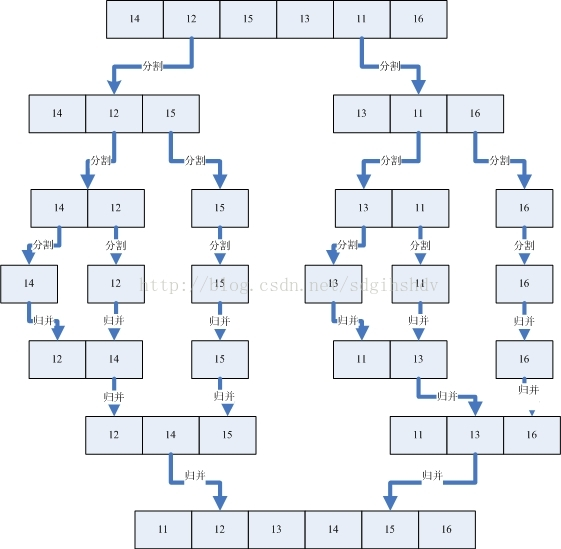
\includegraphics[width=0.75\textwidth]{figs/merge-sort.jpg}
  
\end{frame}

\begin{frame}[fragile]
  \frametitle{归并排序算法分析}
  \begin{easylist} \easyitem
    & 空间复杂度: $O(n)$

    & 在第$i$趟归并后,有序子文件长度为$2^i$ ,因此,因此,对于具有$n$个记录的序列来
    说,需要$ \lceil log_2 n \rceil$趟归并。每趟归并的时间复杂度为$O(n)$。因此,归
    并算法的时间复杂度为$O(n\cdot log_2 n)$

    & 稳定的排序方法
  \end{easylist}
\end{frame}

\begin{frame}[fragile]
  \frametitle{归并排序算法分析}
  \begin{easylist} \easyitem

    & 对于内存排序来说,归并排序的性能不如快速排序那么好,而且它的编程一点也不简单。
    但归并排序是外部排序的中心思想。

    & 在有些情况下,数据集太大而不能完全存储在内存中被处理,此时硬盘读取时间远大于
    内存处理时间。硬盘读取成为制约效率的关键!
  \end{easylist}
\end{frame}

\subsection{基数排序}
\begin{frame}[fragile]
  \frametitle{基数排序}
  \begin{infobox}{算法思想}
    不需要直接对元素进行相互比较,也不需要将元素相互交换,而是对元素进行“分类”。

    如果对效率有所要求,而不太关心空间的使用时,可以选择用计数排序。
  \end{infobox}
\end{frame}

\begin{frame}[fragile]
  \frametitle{Reference}

  \begin{itemize}
  \item 各种排序算法的在线动画演示:

    \url{https://www.cs.usfca.edu/~galles/visualization/ComparisonSort.html}
    
    \url{http://www.atool.org/sort.php}

  \item 搜索排序漫画系列
    \url{https://www.itcodemonkey.com/article/11276.html}
  \end{itemize}
\end{frame}

\begin{frame}[fragile]
  \frametitle{本周作业}
  \begin{itemize}
  \item 编程实现插入排序、希尔排序、冒泡排序、快速排序、选择排序、堆排序和二路归
    并排序。
  \item 能够对相同的一组输入,在一个地方(例如主函数里面)里面分别调用不同的方法,
    并记录每种排序算法各自的运行时间。
  \item 测试序列:27, 38, 1, 10, 27, 38, 3, 6, 9, 11, 18, 27, 9, 5, 100000,
    1000001, 0, 10002220011, 11, 56, 79, 78, 5, 12, 8, 13, 9, 12, 10, 12
  \end{itemize}
\end{frame}